\documentclass{rapportINPTCLOUD}
\usepackage{lipsum}
\usepackage{listings}
\usepackage{color}
\usepackage{biblatex}
\usepackage{appendix}
\usepackage{hyperref}

\definecolor{gray}{rgb}{0.5,0.5,0.5}
\definecolor{lightgray}{rgb}{0.95, 0.95, 0.95}

\fairemarges

\begin{document}

\lstset{
    basicstyle=\ttfamily\small,
    backgroundcolor=\color{lightgray},
    frame=single,
    breaklines=true,
    showstringspaces=false,
    keywordstyle=\color{blue},
    commentstyle=\color{green!60!black},
    stringstyle=\color{red},
    numbers=left,
    numberstyle=\tiny\color{gray},
    captionpos=b,
    inputencoding=utf8,
    extendedchars=true,
    literate={é}{{\'e}}1 {è}{{\`e}}1 {à}{{\`a}}1 {ç}{{\c{c}}}1 {ê}{{\^e}}1 {ë}{{\"e}}1 {î}{{\^i}}1 {ï}{{\"i}}1 {ô}{{\^o}}1 {ù}{{\`u}}1
}

%----------- Informations du rapport ---------

\titre{Rapport de Conception Web : Site MSC INPT}

\sujet{Atelier Développement Web - Session 2}

\Encadrants{\Large M. \textsc{SADIK}} % Assumed generic Prof name based on context, user can change if needed

\eleves{\Large  \textsc{}} % User needs to fill this

%----------- Initialisation -------------------

\fairepagedegarde
\tabledematieres

%----------- Contenu du Rapport ----------------

% Intro
\chapter{Introduction}
Dans le cadre de l'atelier de d\'eveloppement web, ce rapport pr\'esente la conception et le d\'eveloppement d'un site web complet et responsif pour le club Math \& Science Club (MSC) de l'INPT Rabat. L'objectif principal de ce projet \'etait de cr\'eer une plateforme moderne, attrayante et fonctionnelle pour mettre en valeur les activit\'es du club, ses membres et ses \'ev\'enements, notamment les Olympiades 2025.

Pour r\'ealiser ce projet de mani\`ere efficace en tant qu'\'el\`eve ing\'enieur, j'ai choisi d'utiliser \textbf{Bootstrap 5} pour la structure globale (le "grid system") et les composants responsifs, combin\'e \`a du \textbf{CSS Vanilla} (personnalis\'e) pour obtenir une identit\'e visuelle unique (Glassmorphism, d\'egrad\'es, animations fluides). Le \textbf{JavaScript} a \'et\'e utilis\'e pour ajouter des interactions dynamiques comme les compteurs anim\'es et les effets au d\'efilement.

\section{Lien du D\'ep\^ot GitHub}
L'int\'egralit\'e du code source de ce projet (HTML, CSS, JavaScript et les assets) est disponible sur mon d\'ep\^ot GitHub \`a l'adresse suivante :\\
\url{https://github.com/mehdzii/msc_website.git} \\


\chapter{R\'ealisation et Captures d'\'Ecran}

Dans cette section, nous d\'etaillerons les diff\'erentes parties du site web, en expliquant les choix techniques et en illustrant le r\'esultat avec des captures d'\'ecran.

\section{Section Hero : Accueil Dymanique}
La section "Hero" (l'en-t\^ete du site) a \'et\'e con\c{c}ue pour capter imm\'ediatement l'attention. 

\textbf{Explication technique :}
\begin{itemize}
    \item \textbf{Navbar avec Glassmorphism :} J'ai utilis\'e les classes utilitaires de Bootstrap pour fixer la barre de navigation en haut (\texttt{fixed-top}), mais j'ai \'ecras\'e le fond avec du CSS personnalis\'e (\texttt{backdrop-filter: blur()}) pour donner cet effet de verre d\'epoli tr\`es moderne.
    \item \textbf{Le Logo :} Remplacement de l'ancien logo par une version PNG transparente (\texttt{logo.png}) pour une meilleure int\'egration visuelle.
    \item \textbf{Arri\`ere-plan 3D :} Un script Three.js personnalis\'e (\texttt{three-bg.js}) g\'en\`ere des particules math\'ematiques flottantes et interactives, ce qui correspond parfaitement au th\`eme du club MSC.
\end{itemize}

\begin{figure}[h!]
    \centering
    
\includegraphics[width=0.9\textwidth]{images/hero.png}
    \caption{Section Hero avec la barre de navigation Glassmorphism et l'arri\`ere-plan interactif}
\end{figure}

\newpage
\section{Section \'A Propos : Statistiques et Grille Bento}
Cette section pr\'esente les informations cl\'es du club de mani\`ere tr\`es visuelle.

\textbf{Explication technique :}
\begin{itemize}
    \item \textbf{Compteurs de Statistiques (\texttt{stats-row}) :} J'ai cr\'e\'e une rang\'ee avec Flexbox (\texttt{display: flex}) pour aligner les chiffres h\'ero\"\i ques (150+ membres, 25 \'ev\'enements). Un script JavaScript (\texttt{IntersectionObserver}) a \'et\'e impl\'ement\'e pour que les chiffres s'animent et comptent de $0$ \`a leur valeur cible uniquement quand l'utilisateur scrolle jusqu'\`a cette section, rendant la page vivante.
    \item \textbf{Bento Grid :} Pour s'\'eloigner d'une mise en page classique en colonnes Bootstrap, j'ai utilis\'e la grille CSS (\texttt{display: grid}) pour cr\'eer une disposition "Bento". C'est un choix tr\`es tendance en UI design.
    \item \textbf{Carte Mission \& INPT :} La carte Mission dispose d'un fond d\'egrad\'e bleu sombre avec le texte mis en \'evidence via la police \textit{Playfair Display}. La carte INPT utilise une vraie photo du campus (\texttt{inpt.jpeg}) en arri\`ere-plan (\texttt{background-size: cover}) recouverte d'un d\'egrad\'e transparent pour que le texte "View on Maps" (qui est un vrai lien cliquable redirigeant vers Google Maps) reste lisible.
\end{itemize}

\begin{figure}[h!]
    \centering
    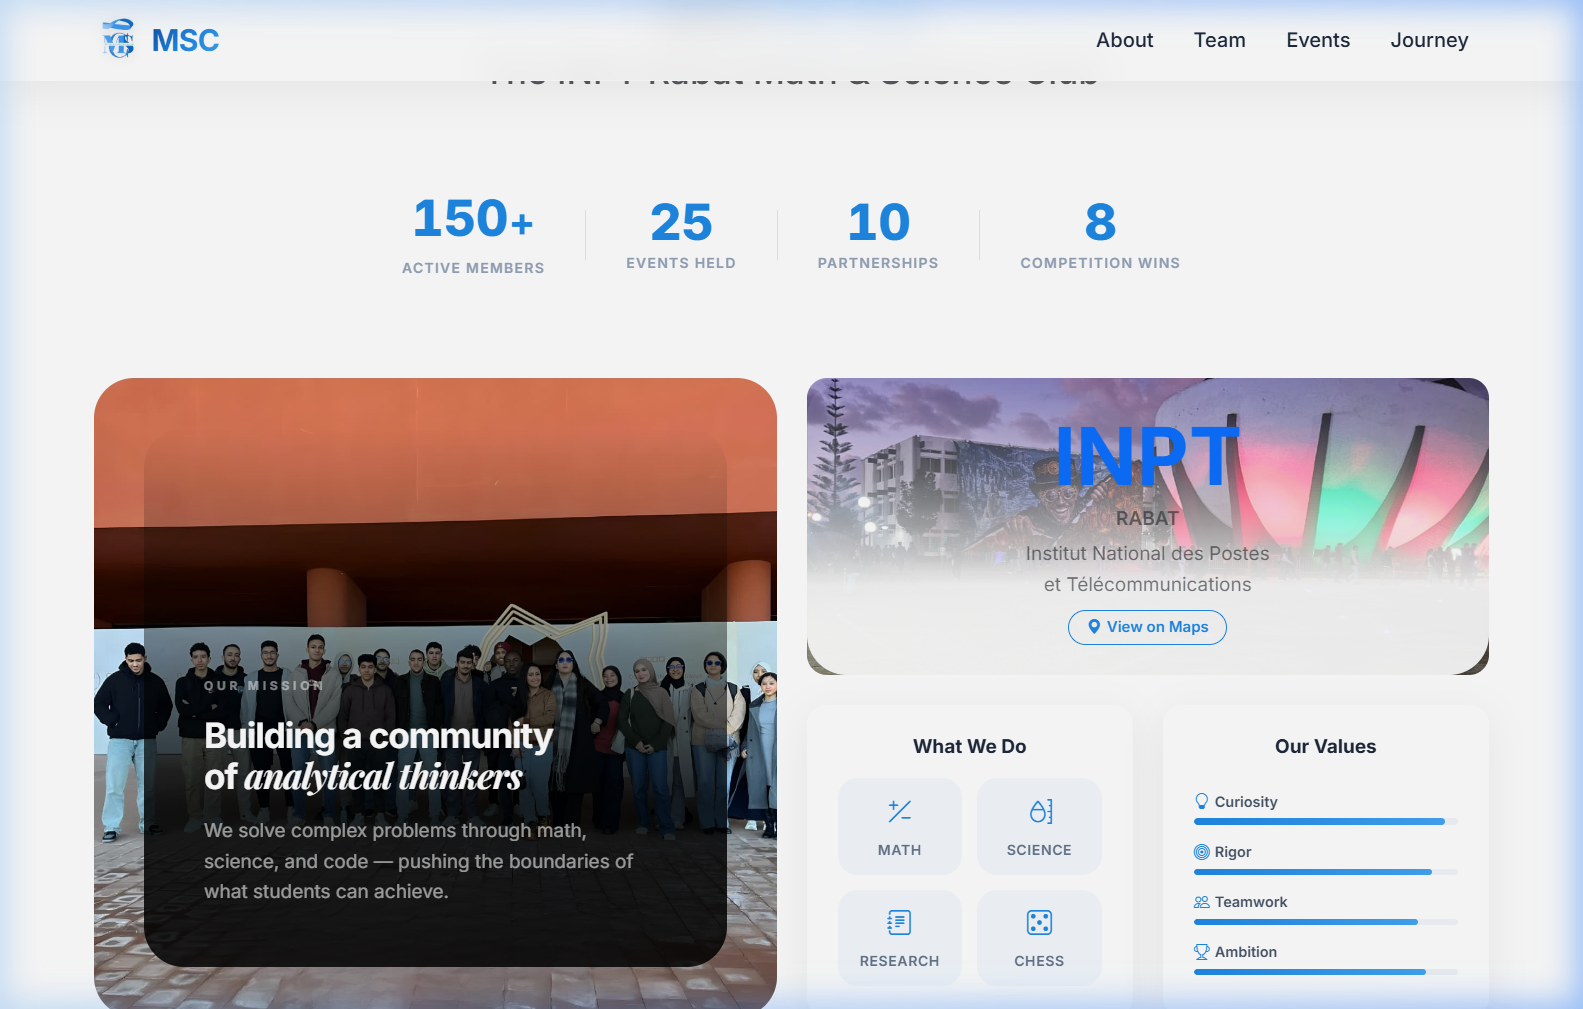
\includegraphics[width=1\textwidth]{images/stats.png}
    \caption{Ligne des statistiques avec les compteurs anim\'es via JavaScript}
\end{figure}

\begin{figure}[h!]
    \centering
    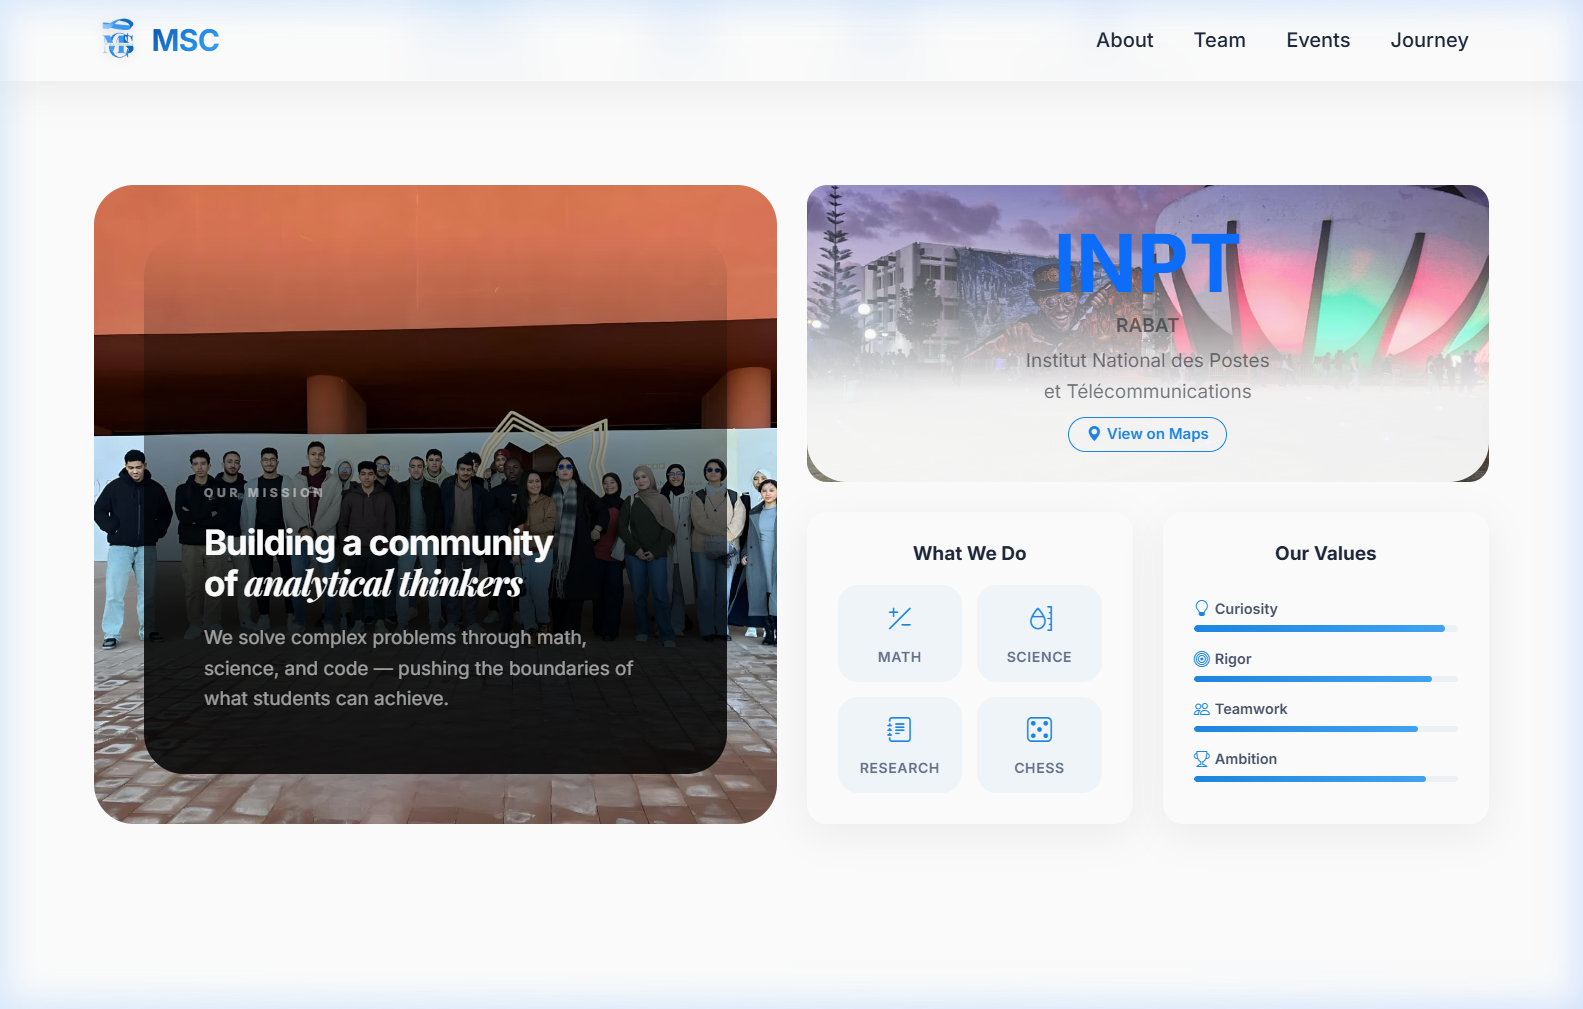
\includegraphics[width=1\textwidth]{images/bento.png}
    \caption{La grille "Bento" affichant la mission, la localisation INPT et nos valeurs}
\end{figure}

\newpage
\section{Section \'Equipe : "The Core"}
Pour pr\'esenter les membres centraux du club, j'ai opt\'e pour un style "\'Editorial" diff\'erent des simples cartes de profil.

\textbf{Explication technique :}
\begin{itemize}
    \item \textbf{Collage Asym\'etrique :} Utilisation de CSS Grid pour positionner les images des membres (President, Vice-President, etc.) dans une composition asym\'etrique qui ressemble \`a une page de magazine.
    \item \textbf{Filtres CSS :} Les portraits sont en noir et blanc (gr\^ace \`a \texttt{filter: grayscale(100\%)}). Lorsqu'on survole un membre, l'image transitionne vers ses couleurs d'origine, apportant de l'interactivit\'e.
    \item \textbf{D\'egrad\'es Invers\'es :} Au lieu d'encadrer les photos, le texte est s\'epar\'e par des lignes fines et d\'ecale les images, avec des badges subtils (ex: "VISION \& STRATEGY").
\end{itemize}

\begin{figure}[h!]
    \centering
    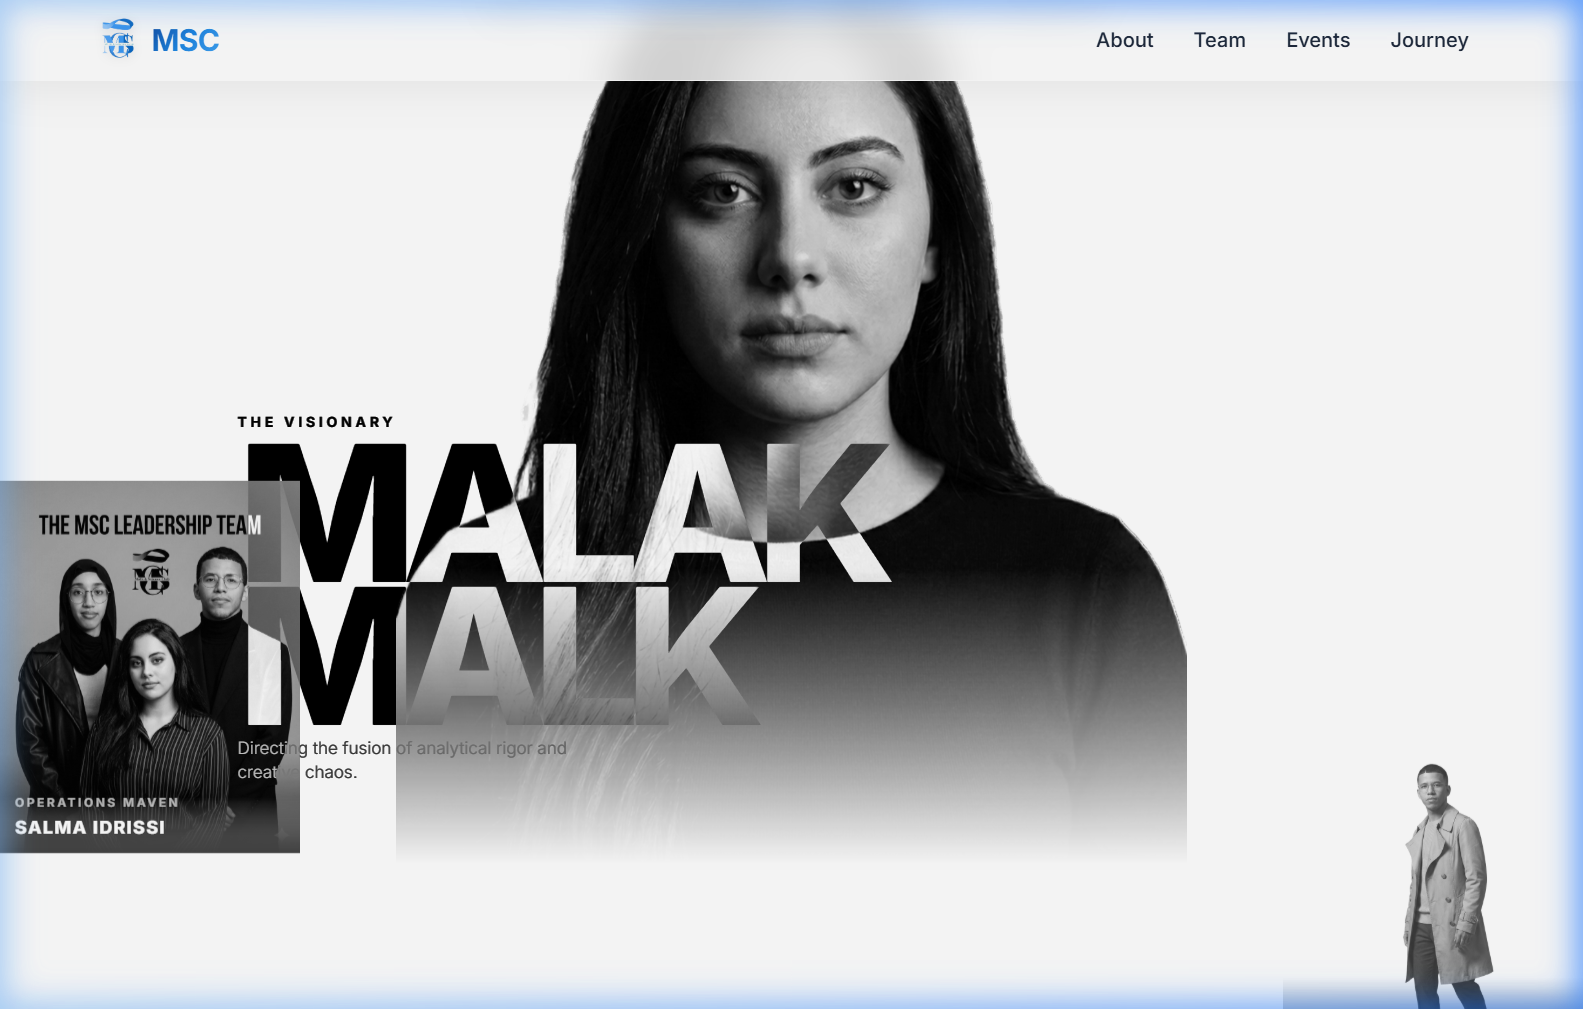
\includegraphics[width=0.9\textwidth]{images/team.png}
    \caption{Section de l'\'equipe avec son style \'editorial asym\'etrique}
\end{figure}

\newpage
\section{Section \'Ev\'enements : D\'efilement Horizontal Infinity}
Le club organise beaucoup d'\'ev\'enements. Il fallait les pr\'esenter de fa\c{c}on optimis\'ee.

\textbf{Explication technique :}
\begin{itemize}
    \item \textbf{Carrousel \`a D\'efilement Horizontal :} Pour \'eviter que la page ne devienne trop longue, la galerie d'\'ev\'enements d\'efile horizontalement infiniment gra\^ce \`a quelques lignes de JavaScript calculant le scroll et clonant les \'el\'ements \texttt{scroll-track}.
    \item \textbf{Olympiades 2025 (Timer) :} Pour l'\'ev\'enement phare, j'ai int\'egr\'e un compte \`a rebours circulaire mis \`a jour en temps r\'eel via JS, calculant les jours/heures/minutes avant l'\'ev\'enement.
    \item Les images pertinentes (\texttt{math\_trivia.jpg}, \texttt{battle\_royale.jpg}, \texttt{colloque.jpg}) ont \'et\'e li\'ees aux cartes correspondantes pour donner du contexte.
\end{itemize}

\begin{figure}[h!]
    \centering
    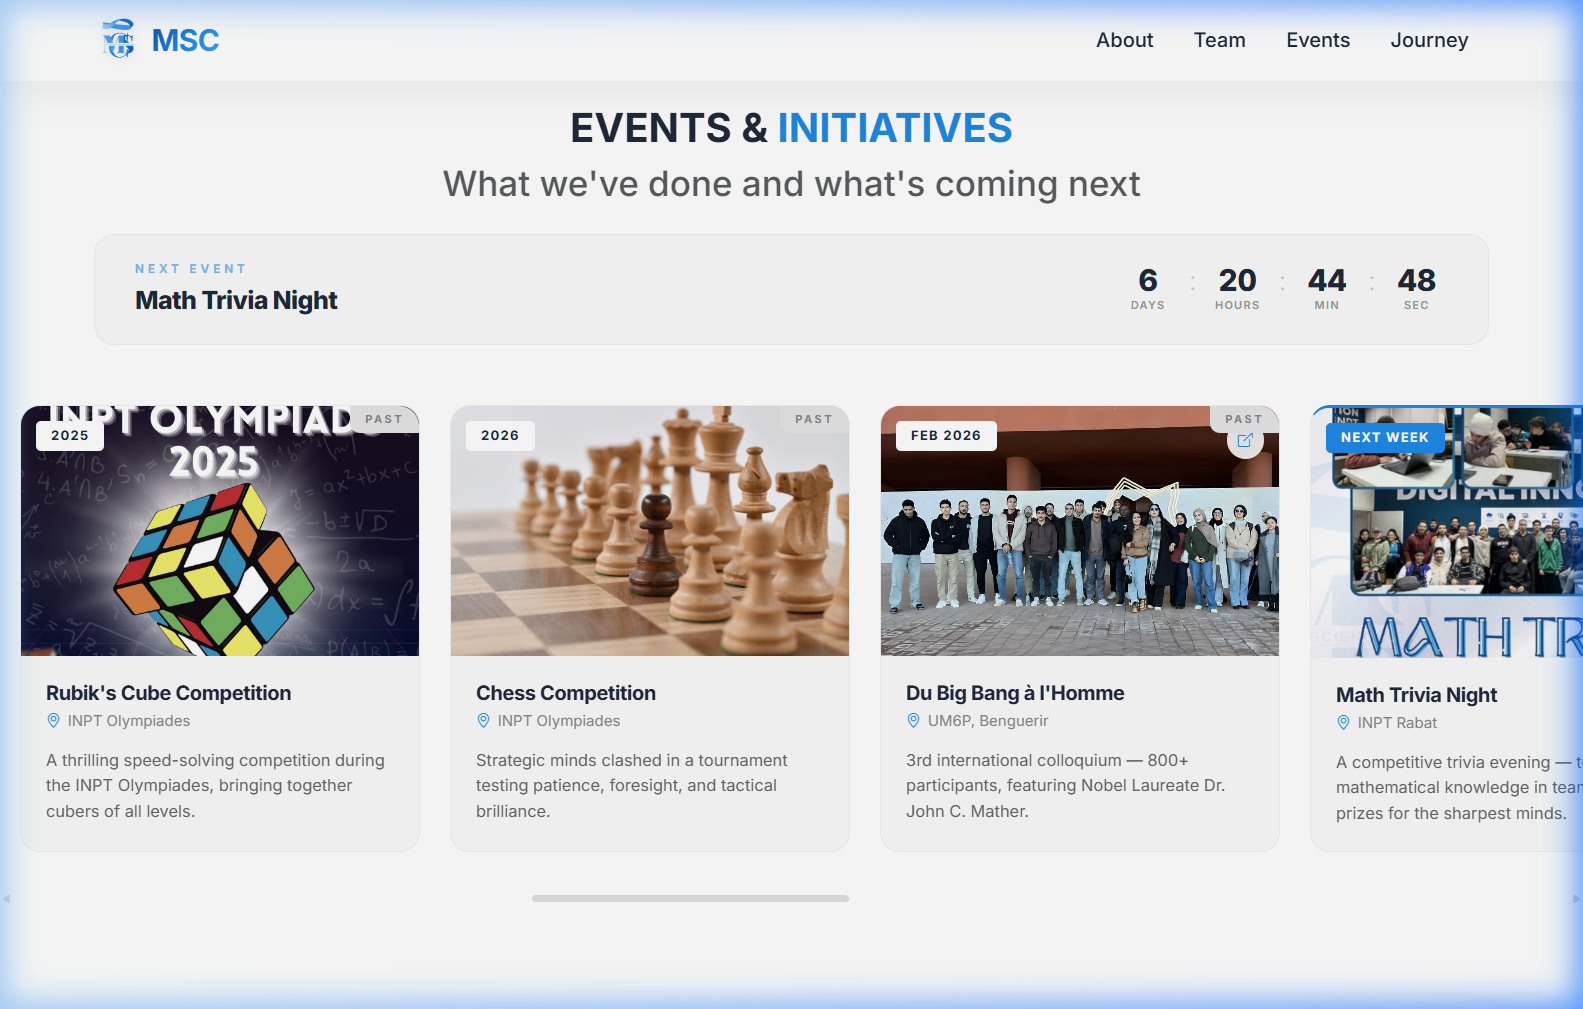
\includegraphics[width=1\textwidth]{images/events.png}
    \caption{Galerie d'\'ev\'enements avec d\'efilement infini et timer adaptatif}
\end{figure}

\newpage
\section{Le Footer (Pied de page)}
Le footer cl\^oture le site avec nettet\'e et une navigation utile.

\textbf{Explication technique :}
\begin{itemize}
    \item \textbf{Liens Sociaux Fonctionnels :} Remplacement des id\'ees al\'eatoires par de vrais ic\^ones Bootstrap cliquables qui m\`enent aux vrais r\'eseaux du club MSC (Instagram, LinkedIn) et au challenge Cicada sur Proton Drive.
    \item \textbf{Rendu SVG :} Le logo complet a \'et\'e int\'egr\'e en noir et mis en page de fa\c{c}on tr\`es \'epur\'ee, toujours en gardant la charte graphique bleue (\texttt{\#1E88E5}) au survol des liens.
\end{itemize}

\begin{figure}[h!]
    \centering
    
\includegraphics[width=1\textwidth]{images/footer.png}
    \caption{Le footer minimaliste contenant les liens de r\'eseaux sociaux et copyrights}
\end{figure}

\chapter{Organisation du Code \& Commentaires}
Un point d'honneur a \'et\'e mis sur la "propret\'e" du code, une comp\'etence essentielle pour le travail en \'equipe. 
\begin{enumerate}
    \item \textbf{Fichier CSS comment\'e (\texttt{style.css}):} Le fichier est d\'ecoup\'e en chapitres logiques (ex: \texttt{1. Base \& Typography}, \texttt{4. Hero Section}, \texttt{12. Stats Counter Row}, etc.). Toutes les couleurs "violettes" obsol\`etes ont \'et\'e identifi\'ees via les variables CSS (\texttt{--accent-primary}) et modifi\'ees globalement en un th\`eme bleu l\'eger (\texttt{\#1E88E5}).
    \item \textbf{JavaScript document\'e (\texttt{main.js}):} Les fonctions de scroll, le timer et le compte \`a rebours circulaire poss\`edent toutes des commentaires explicatifs JSDoc.
    \item \textbf{Refonte du Formulaire :} Un formulaire annexe (\texttt{form/index.html}) a \'et\'e totalement recod\'e. Initialement tr\`es neutre, il a \'et\'e r\'eint\'egr\'e dans le th\`eme global (layout en $2$ colonnes, ombres l\'eg\`eres, boutons aux bords arrondis ou "pills").
\end{enumerate}

\chapter{Conclusion}
Ce projet m'a permis d'assimiler les m\'ecanismes avanc\'es d'un framework (Bootstrap) tout en comprenant ses limites, d'o\`u la n\'ecessit\'e cruciale de ma\^itriser le CSS pur pour cr\'eer des designs r\'ellement "Premium" (effets de flou, grilles personnalis\'ees asym\'etriques). 

L'int\'egration du JavaScript, au travers de requ\^etes \texttt{requestAnimationFrame} pour les compteurs statistiques et l'\texttt{IntersectionObserver} pour les animations au d\'efilement, montre que les comp\'etences logiques acquises en algorithmique sont fondamentales pour dynamiser des interfaces web modernes.

\end{document}
